\chapter{Implementation Design}
\label{chaptImplementation}
In this chapter, we will introduce the implementation of our demo game and explain the basic principles and algorithms behind it. We will try to explain the algorithms and procedures to the maximum extent while avoiding detailing used technology.
\todo {mention measurements}

After consideration of the various approaches implemented in games and also proposed efficient solutions to the problem of real-time destructible environment, we decided to implement a slightly different approach. Our implementation will borrow already tested techniques from multiple approaches.

Our approach is mostly similar to \emph{Geomod} (described in \cref{sec:common}) and \emph{Real Time Dynamic Fracture
with Volumetric Approximate Convex Decompositions}(RTDF) (described in \cref{sec:RTDF}) with a key differences. 

\section{Main algorithm}
Our approach generates Voronoi cell at the point of collision. Then the difference of original mesh and the Voronoi cell is calculated and represents the damaged object. To generate the debris the intersection of original mesh and the Voronoi cell is calculated. This action effectively cuts the object into two or more pieces, all of which are put back into simulation and can be damaged again (see \cref{fig:subtraction}). The Voronoi cell was our choice of shape because it has easily randomizable shape and provides aesthetically good looking results. The shape is in no way critical to the rest of algorithm and can be changed for any closed mesh.

Similarly to the RTDF approach, the cost of fracturing in our implementation is solely dependent on the size and complexity of the fractured object. \todo{odkaz na merania} This makes the method suitable for use in computer games and real-time simulations.

\begin{figure}
        \centering
        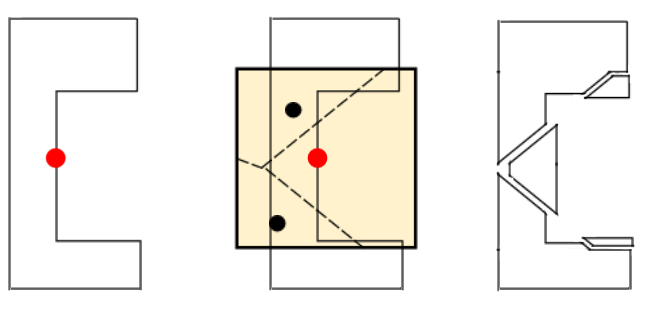
\includegraphics[width=\textwidth]{img/subtractionProcess}
        \caption{object with point of impact (left), generated Voronoi cell (centre), object divided into six new smaller objects after subtraction of Voronoi cell (right)}
        \label{fig:subtraction}
\end{figure}

Randomization of the size and shape of a Voronoi cell makes the game look more realistic because it guarantees different result after every collision. The generation of a Voronoi cell takes place in a closed domain with its centre at the point of collision. In the domain, in addition to the centre point, random points need to be generated. The used Voronoi cell is the cell of the centre point cut by the boundaries of the domain if necessary.

We also considered implementation based on \emph{A fast method for simulating destruction and the generated dust and debris} (see \cref{sec:edem}). To test this approach, we set up a cube divided into 439 tetrahedrons. After introducing constraints to hold the tetrahedrons together, we experienced a drop from 60fps (set as an upper limit) to 13fps. Having a large number of elements connected with springs in the simulation can also trigger an undesirable behaviour (contractions and retractions, object blowing up). Performance issues and problems with keeping elements in a stable state concludes that this approach is not suitable for our work.




\section{Program Structure}
Disregarding the initialization, the program runs in following steps:
\begin{enumerate}
\item Perform a step in physics simulation.
\item Handle collisions and perform destruction, see \cref{sec:collisions}.
\item Read user input and then apply correct forces to controlled vehicle.
\item Render current state of objects. In this step, a graphical representation of every object is updated to comply with its rigid body version.
\end{enumerate}

\begin{figure}
        \centering
        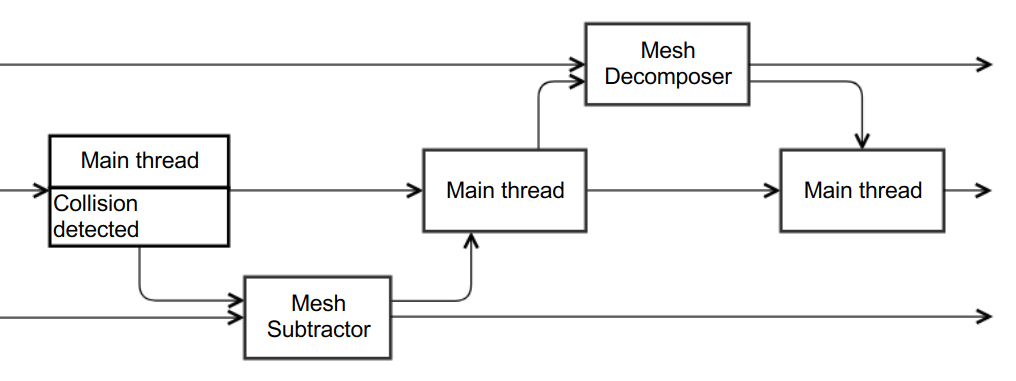
\includegraphics[width=\textwidth]{img/decompositionFlow}
        \caption{Diagram is showing multiple threads handling collision event. }
        \label{fig:threads}
\end{figure}
To make our application faster, we can execute the most costly tasks asynchronously in separate threads. Those tasks are convex decomposition and mesh subtraction. As a result, the program is running in three threads (\cref{fig:threads}): the main thread, a thread for subtracting meshes and a thread for decomposing triangular mesh into a set of convex shapes (\cref{sec:decomposition}). Both subtraction and decomposition threads communicate solely with the main thread, and all communication is done in producer-consumer model. Figure \ref{fig:objectInThreads} shows the changes of the object and its collision shape across all threads.

\begin{figure}
        \centering
        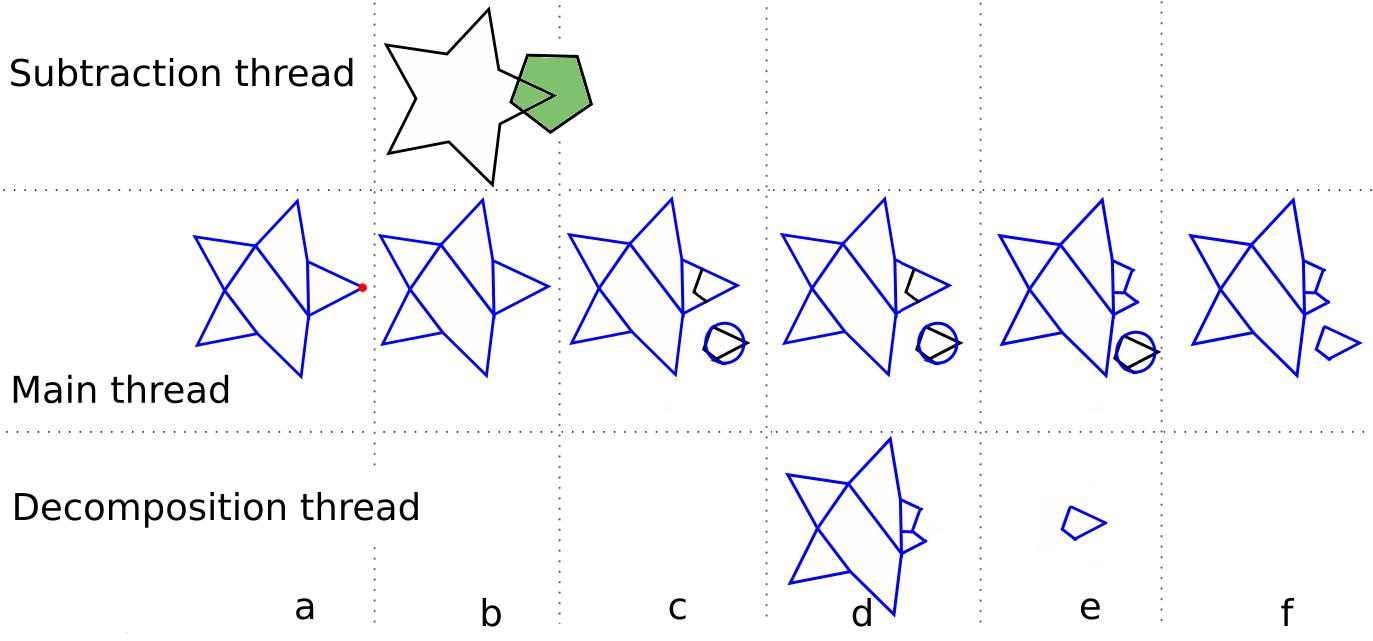
\includegraphics[width=\textwidth]{img/object-progress}
        \caption{The figure shows a simplified overview of changing states of a single object across multiple threads in simultaneous time slots. We can see the process of splitting the mesh and calculation of collision shapes from the time of the collision until the convex decomposition is calculated for all parts. The blue lines represent a collision shape. Black represents a visual mesh and the red dot collision point. If the collision shape matches the visual mesh, only the shape is shown. }
        \label{fig:objectInThreads}
\end{figure}

\section{Collision handling}
\label{sec:collisions}
After the collision, we get a reference to two rigid bodies participating in the collision, point of collision and vector of force from the physics engine. For simplification, we will consider only one object, the point of impact and the force.

At first, we need to filter out unwanted collisions (collisions that should not damage the object). Those collisions can be results of an object placed on ground or collisions with not enough force to damage the object. 

For every valid collision, we will generate Voronoi cell as described earlier and put meshes of both objects into a task for mesh subtraction thread. After enqueuing all collisions, we can check if there are any prepared subtraction results for further use. The result of one subtraction task is a set of meshes that represent new objects. For every mesh, we create a new object, but we do not have its convex decomposition for the physics engine to perform accurate collision detection. Because decomposition can take long, we will create simple temporary collision shape (\eg sphere) and a task for decomposition. Then we will proceed with simulation, not waiting for the result. Decomposition is done in a separate thread, and the result is returned to the main thread where we check for decomposed shapes. With the shape ready in the main thread we replace the temporary shape for compound shape consisting of convex parts.

This process guarantees that we do not wait for either subtraction or decomposition and therefore we can have stable fps in our game. Temporarily replacing a collision shape by a simpler alternative ensures consistent behaviour of new objects (we can put them into the simulation, and they do not fall through each other or otherwise not comply with laws of physics). Therefore we need to calculate the difference of meshes in a period of a few frames so it can not be seen that it is lagging behind collisions.

\section{Convex Decomposition}
\label{sec:decomposition}
Regardless of used physics engine, our objects are represented as triangular meshes. It means that to perform accurate mesh to mesh collisions, every object needs to have its collision shape in the form of compound shape consisting of convex bodies. While it is desirable to have a decomposition into a minimum number of pieces, this problem is known to be NP-hard \cite{convexDecomp}. 

In the setting of a computer game, the speed of calculation is much more relevant than the precision. The small differences between collision shapes and visual meshes are not considered to be a problem. The important part is to be able to perform collisions at real-time. A number of approximate convex decomposition algorithms have been proposed to solve this problem.

We have chosen to use \emph{Hierarchical Approximate Convex Decomposition} algorithm (see \cref{sec:decompositionLib}). The application designed in such way that after every mesh subtraction convex decomposition needs to be applied to the rest of the original mesh and every new part.

\section{Measurements???}
\todo{nieco rozumne namerat a napisat o tom}

